% !TeX program = xelatex
% !TeX encoding = UTF-8
% Сборка из каталога docs: xelatex field-reconstruction-report.tex (дважды).
\documentclass[a4paper,11pt]{article}

% pdfLaTeX использует T2A; XeLaTeX/LuaLaTeX — Unicode-шрифты.
\usepackage{iftex}
\ifPDFTeX
  \usepackage[T2A]{fontenc}
  \usepackage[utf8]{inputenc}
  \usepackage[english,russian]{babel}
\else
  \usepackage{fontspec}
  \usepackage{polyglossia}
  \setdefaultlanguage{russian}
  \setotherlanguage{english}
  \setmainfont{Libertinus Serif}
  \newfontfamily\cyrillicfont{Libertinus Serif}
\fi

\usepackage[top=16mm,bottom=16mm,left=18mm,right=18mm]{geometry}
\usepackage{amsmath,amssymb}
\usepackage{graphicx}
\usepackage{booktabs,tabularx,array}
\usepackage{caption}
\usepackage{titlesec}
\usepackage[hidelinks,unicode]{hyperref}

\graphicspath{{screenshots/}}
\hypersetup{pdftitle={Восстановление магнитного поля в объёме TPC}}
\titleformat{\section}{\large\bfseries}{\thesection}{0.6em}{}
\titlespacing*{\section}{0pt}{0pt}{10pt}
\captionsetup{font=small,labelfont=normalfont,labelsep=space}
\setlength{\parindent}{0pt}
\setlength{\parskip}{6pt}
\setlength{\abovedisplayskip}{8pt}
\setlength{\belowdisplayskip}{8pt}
\renewcommand{\arraystretch}{1.25}
\newcolumntype{C}{>{\centering\arraybackslash}X}
\DeclareMathOperator*{\argmin}{arg\,min}

\begin{document}

{\Large\bfseries Восстановление магнитного поля в объёме TPC\par}
\vspace{4pt}

\section{Постановка задачи и физическая модель}

\textbf{Назначение расчёта.} Требуется восстановить три компоненты магнитного
поля внутри цилиндрического объёма TPC по ограниченному набору измерений
на его торцах. 12 трёхкомпонентных датчиков E1\ldots E6 и W1\ldots W6
дают 36 значений $B_r$, $B_\varphi$ и $B_z$. Радиус области — 1408,569~мм,
длина — 4058~мм; торцы находятся при $z=\pm2029$~мм. Номинальное поле —
5000~Гс, или 0,5~Тл. Координаты задаются в миллиметрах, поле — в гауссах.

Напряжения преобразуются по индивидуальным коэффициентам
$B=k(V-V_0)$, где $V,V_0$ выражены в мВ, $k$ — в Гс/мВ.
Данные поступают через OPC UA. Компоненты R/F/Z должны быть приведены
к общей цилиндрической системе TPC; неверная ориентация или знак канала
не исправляются самим методом восстановления.

\textbf{Ограничения Максвелла.} В области без токов при постоянной магнитной
проницаемости принимаются условия
\[
 \nabla\cdot\mathbf B=0,\qquad \nabla\times\mathbf B=0.
\]
В односвязной области можно ввести скалярный потенциал:
$\mathbf B=-\nabla\Phi$. Тогда первое условие даёт уравнение Лапласа
$\nabla^2\Phi=0$. Это обосновывает выбор гармонических полиномиальных мод:
они связывают компоненты поля физическими условиями, а не аппроксимируют
каждую компоненту независимо.

Вводятся безразмерные координаты $\rho=r/L$, $\zeta=z/L$,
где $L=\max_i\{|r_i|,|z_i|\}$. Угол $\varphi$ не масштабируется.
Один общий масштаб для $r$ и $z$ сохраняет гармонические свойства.
Реализованная модель имеет вид
\[
 \mathbf B(r,\varphi,z)=\sum_{k=0}^{9}c_k\mathbf f_k(\rho,\varphi,\zeta).
\]
Компоненты десяти мод приведены ниже; коэффициенты $c_k$ имеют единицы поля.

\begin{center}
\small
\begin{tabular}{c c c c}
\toprule
$k$ & $f_{k,r}$ & $f_{k,\varphi}$ & $f_{k,z}$ \\
\midrule
0 & $0$ & $0$ & $1$ \\
1 & $-\rho/2$ & $0$ & $\zeta$ \\
2 & $-\rho\zeta$ & $0$ & $\zeta^2-\rho^2/2$ \\
3 & $-3\rho\zeta^2/2+3\rho^3/8$ & $0$ & $\zeta^3-3\rho^2\zeta/2$ \\
4 & $\cos\varphi$ & $-\sin\varphi$ & $0$ \\
5 & $\sin\varphi$ & $\cos\varphi$ & $0$ \\
6 & $\zeta\cos\varphi$ & $-\zeta\sin\varphi$ & $\rho\cos\varphi$ \\
7 & $\zeta\sin\varphi$ & $\zeta\cos\varphi$ & $\rho\sin\varphi$ \\
8 & $\rho\cos2\varphi$ & $-\rho\sin2\varphi$ & $0$ \\
9 & $\rho\sin2\varphi$ & $\rho\cos2\varphi$ & $0$ \\
\bottomrule
\end{tabular}
\end{center}

Мода 0 задаёт однородное продольное поле; моды 1--3 описывают
осесимметричные изменения, 4--5 — однородное поперечное поле,
6--7 — связанные продольные и поперечные изменения, 8--9 — поперечную
квадрупольную структуру. Базис регулярный на оси при записи в декартовых
координатах. Десять мод ограничивают класс восстанавливаемых полей:
36 измерений сами по себе не определяют произвольную функцию в объёме.

\clearpage
\section{Обратная задача и определение коэффициентов}

\textbf{Матрица измерений.} Для каждого датчика $i=0,\ldots,11$
и компоненты $\alpha\in\{r,\varphi,z\}$ формируется одна строка системы.
Если номер компоненты $q$ равен 0, 1 или 2, то
\[
 A_{3i+q,k}=f_{k,\alpha}(r_i/L,\varphi_i,z_i/L),\qquad
 b_{3i+q}=B_{i,\alpha}^{\mathrm{meas}}.
\]
Матрица $A$ имеет размер $36\times10$, вектор $\mathbf b$ — 36 элементов.
Все три компоненты одного датчика участвуют в общем определении
коэффициентов. Система переопределена, поэтому при шуме измерений
точного равенства $A\mathbf c=\mathbf b$ обычно нет.

Используется невзвешенный метод наименьших квадратов:
\[
 \widehat{\mathbf c}=\argmin_{\mathbf c}
 \|A\mathbf c-\mathbf b\|_2^2.
\]
Все каналы имеют одинаковый вес. Индивидуальные неопределённости измерений
в текущем решении не задаются. Нормальные уравнения
$A^{\mathsf T}A\mathbf c=A^{\mathsf T}\mathbf b$ описывают условие минимума,
но непосредственно не используются: образование $A^{\mathsf T}A$
возводит число обусловленности в квадрат.

\textbf{Нормировка и SVD.} Для уменьшения влияния разных порядков полиномов
каждый столбец делится на свою евклидову норму:
\[
 s_k=\|A_{:,k}\|_2,\quad D=\operatorname{diag}(s_0,\ldots,s_9),\quad
 \widetilde A=AD^{-1},\quad \mathbf d=D\mathbf c.
\]
В библиотеке Eigen выполняется сингулярное разложение
$\widetilde A=U\Sigma V^{\mathsf T}$.
При полном ранге решение и обратное масштабирование записываются как
\[
 \widehat{\mathbf d}=
 \sum_{\ell=1}^{10}\frac{\mathbf u_\ell^{\mathsf T}\mathbf b}{\sigma_\ell}
 \mathbf v_\ell,\qquad
 \widehat{\mathbf c}=D^{-1}\widehat{\mathbf d}.
\]
Сингулярные значения упорядочены:
$\sigma_1\geq\cdots\geq\sigma_{10}\geq0$.
Численный ранг определяется относительным порогом $10^{-10}$;
значения ниже порога относительно $\sigma_1$ не используются при решении.
Полный ранг равен 10. Это численный критерий наблюдаемости мод,
а не требование к однородности магнитного поля.

При нулевой норме столбца соответствующая мода не наблюдается датчиками.
Строгий режим отклоняет такую систему или неполный ранг.
В режиме предупреждений нулевая норма заменяется единицей,
и SVD даёт решение минимальной нормы в переменных $\mathbf d$
по сохранённым сингулярным направлениям. Такое решение предварительное:
неопределённые измерениями моды не становятся физически известными.

Для полного ранга диагностируется
$\kappa_2(\widetilde A)=\sigma_1/\sigma_{10}$; при неполном ранге
выдаётся бесконечная обусловленность. Возмущение данных передаётся
в коэффициенты по закону $\delta\mathbf d=\widetilde A^+\delta\mathbf b$.
Малые сингулярные значения усиливают шум. Даже хорошая обусловленность
не исключает систематическую ошибку калибровки или недостаточность базиса.
После нахождения коэффициентов поле вычисляется в любой допустимой
точке подстановкой в сумму мод, без повторного решения системы.

\clearpage
\section{Опорная карта, диагностика и получение результата}

\textbf{Коррекция карты.} Если имеется ранее измеренная карта $\mathbf B_0$,
то восстанавливается изменение относительно неё. В точках датчиков
формируется $\Delta\mathbf b_i=\mathbf B_i^{\mathrm{meas}}-\mathbf B_0(\mathbf x_i)$,
а та же матрица $A$ используется для подгонки поправки. Итоговое поле:
\[
 \mathbf B(\mathbf x)=\mathbf B_0^{\mathrm{interp}}(\mathbf x)
       +\sum_{k=0}^{9}\Delta c_k\mathbf f_k(\mathbf x).
\]
Здесь аргумент мод означает соответствующие нормированные цилиндрические
координаты. Без опорной карты коэффициенты описывают всё поле, а не поправку.
Такой режим полезен для предварительной оценки, но не заменяет коррекцию
экспериментально снятой карты.

Карта хранится на декартовой сетке с компонентами $B_x,B_y,B_z$.
При сравнении с датчиками выполняется преобразование
\[
 B_r=B_x\cos\varphi+B_y\sin\varphi,\quad
 B_\varphi=-B_x\sin\varphi+B_y\cos\varphi.
\]
Продольная компонента не меняется. Внутри ячейки поле интерполируется
по восьми вершинам. Для локальных координат $t_x,t_y,t_z\in[0,1]$:
\[
 \mathbf B_0^{\mathrm{interp}}=
 \sum_{a,b,c\in\{0,1\}}w_a(t_x)w_b(t_y)w_c(t_z)\mathbf B_{abc},
 \qquad w_0(t)=1-t,\quad w_1(t)=t.
\]
Выход за границы карты запрещён. Гармоническая поправка удовлетворяет
условиям Максвелла; трилинейная интерполяция самой карты не гарантирует
нулевые дивергенцию и ротор. Эти свойства итогового поля зависят также
от исходной карты и требуют отдельной проверки.

\textbf{Согласованность с датчиками.} По вектору невязок
$\mathbf e=A\widehat{\mathbf c}-\mathbf b$ вычисляются
\[
 e_{\max}=\max_{j=1,\ldots,36}|e_j|,\qquad
 e_{\mathrm{RMS}}=\sqrt{\frac{1}{36}\sum_{j=1}^{36}e_j^2}.
\]
Порог максимальной невязки — 0,2~Гс. В строгом режиме превышение
отклоняет расчёт, в интерактивном — сопровождается предупреждением.
В режиме коррекции невязка относится к разности с картой и одновременно
характеризует совпадение итогового поля с измерениями в датчиках.

\textbf{Проверка в объёме.} В узлах рассчитываются модуль поля
$|\mathbf B|=\sqrt{B_x^2+B_y^2+B_z^2}$ и отношения
\[
 \eta_r=\max_{\mathrm{grid}}\left|\frac{B_r}{B_z}\right|,
 \qquad
 \eta_\perp=\max_{\mathrm{grid}}\frac{\sqrt{B_x^2+B_y^2}}{|B_z|}.
\]
Для $\eta_r$ установлен предел $5{,}2\cdot10^{-4}$.
При $|B_z|<1$~Гс критерий неопределён; на оси вместо неоднозначной
радиальной компоненты используется модуль поперечного поля.
Максимум по узлам не является доказанным максимумом в непрерывном объёме.

Результат формируется как расчётный снимок: объёмная сетка, срезы X/Y/Z
и экспорт VTK. Увеличение плотности сетки уточняет визуализацию и выборочную
оценку экстремумов, но не добавляет измерительной информации.
Малая невязка подтверждает согласованность с датчиками, а не абсолютную
точность: для неё нужны независимые измерения, учёт калибровки,
ориентации, координат датчиков и неопределённости опорной карты.

\clearpage
\section{Результаты проверки}

Научные тесты выполнены в Release на macOS arm64 с Clang 23.1.3.
\textbf{Все 87 проверочных условий прошли:} восстановление гармонических
мод, сохранение ранга при масштабировании, проверки div/curl,
коррекция опорной карты, обработка некорректных данных, срезы и экспорт.

Дополнительный эксперимент выполнен на известном десятимодовом поле.
Датчики размещены при $r = 4$~мм, $z = \pm 3{,}5$~мм,
по шесть на окружности. В 36 каналов добавлялось возмущение
$\delta b_j = \varepsilon \sin(1{,}7j)$.
Восстановление сравнивалось с точным полем в 3349 контрольных узлах.

\begin{center}
  \small
  \begin{tabularx}{\textwidth}{CCC}
    \toprule
    Амплитуда $\varepsilon$, Гс & Максимальная невязка, Гс &
      Максимальная ошибка в объёме, Гс \\
    \midrule
    0    & $1{,}82 \cdot 10^{-12}$ & $2{,}73 \cdot 10^{-12}$ \\
    0,05 & 0,068504 & 0,028609 \\
    0,10 & 0,137008 & 0,057218 \\
    0,20 & 0,274016 & 0,114436 \\
    \bottomrule
  \end{tabularx}
\end{center}

Во всех случаях ранг равен 10, обусловленность нормированной
матрицы — 1,34863. При $\varepsilon = 0{,}20$~Гс строгий режим отклоняет
расчёт из-за невязки выше 0,2~Гс; строка получена в режиме предупреждений.

При отсутствии возмущений ошибка близка к уровню машинного округления.
Для заданного профиля возмущения удвоение $\varepsilon$ удваивает невязку
и ошибку в объёме, что согласуется с линейностью восстановления.
Эти значения характеризуют данный синтетический эксперимент:
они не являются оценкой ошибки для произвольного шума или реального магнита.

\begin{center}
  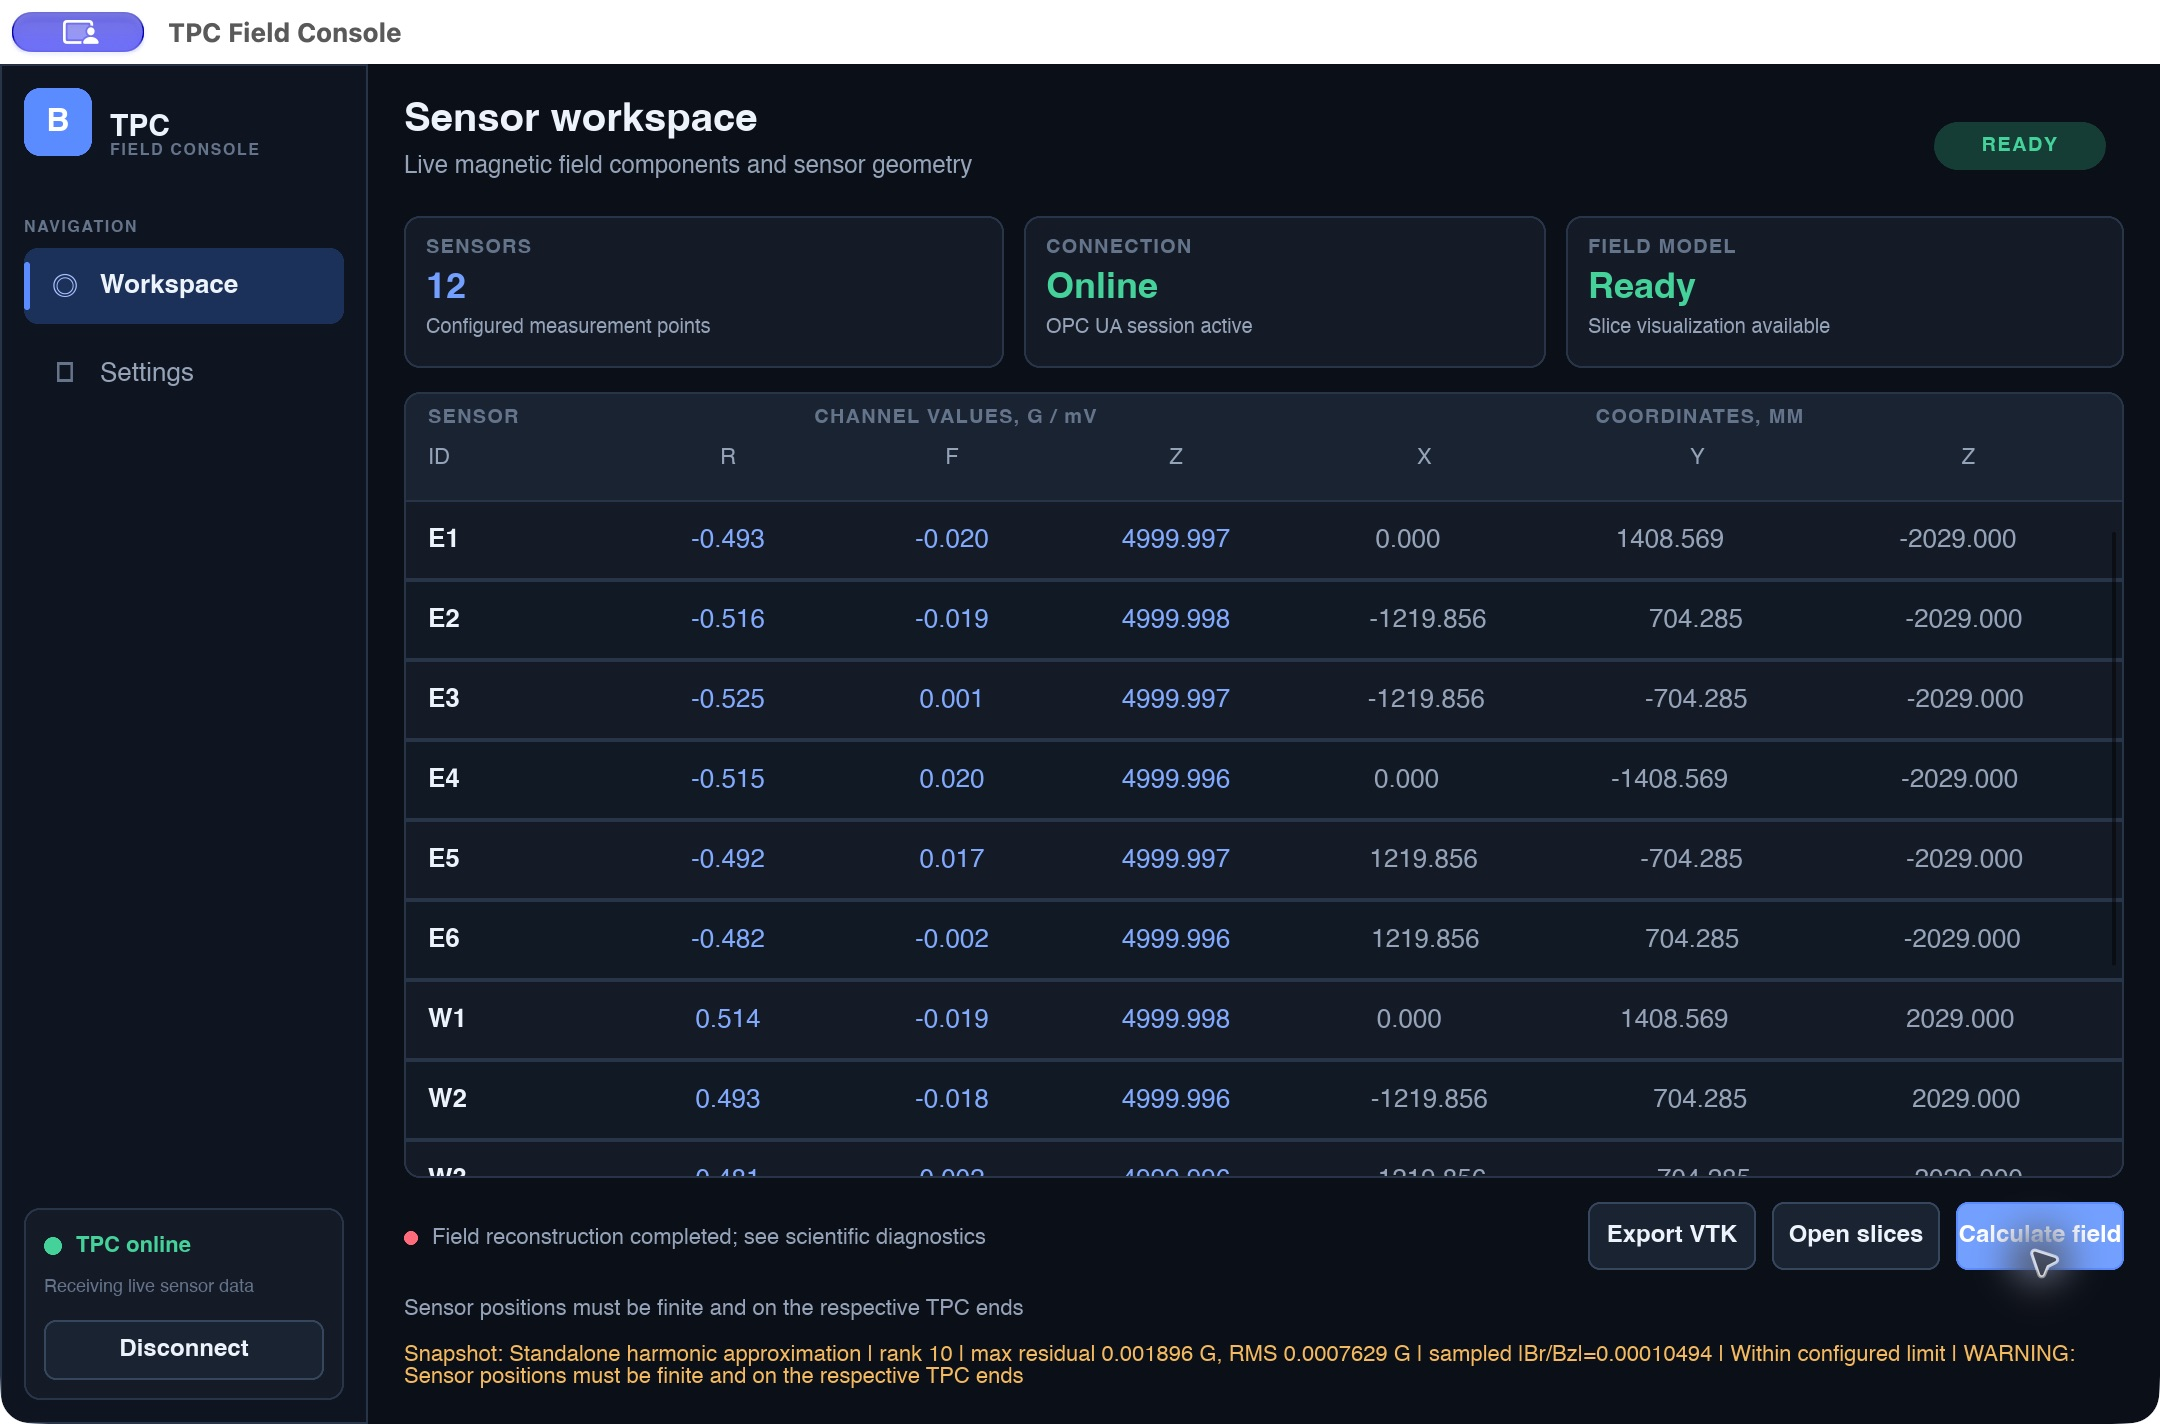
\includegraphics[width=\textwidth]{03-reconstruction.jpg}
  \captionof{figure}{Результат расчёта в TPC Field Console на синтетических
    данных локального OPC UA-сервера.}
  \label{fig:reconstruction}
\end{center}

На снимке: ранг 10, max невязки 0,001896~Гс, RMS 0,0007629~Гс,
$\max |B_r/B_z| = 1{,}0494 \cdot 10^{-4}$.
Значение ниже порога $5{,}2 \cdot 10^{-4}$, но выше $10^{-4}$.
Предупреждение о координатах датчиков сохранено; расчёт выполнен
в предварительном режиме на сетке $32 \times 32 \times 32$, без опорной карты.

\clearpage
\section{Срезы восстановленного поля}

Срезы относятся к расчётному снимку на рисунке~\ref{fig:reconstruction}.
Цвет показывает модуль поля $|\mathbf{B}|$; шкала отдельно нормируется
для каждого среза. Данные синтетические, не являются измерениями магнита MPD.

\begin{center}
  \begin{minipage}{115mm}
    \centering
    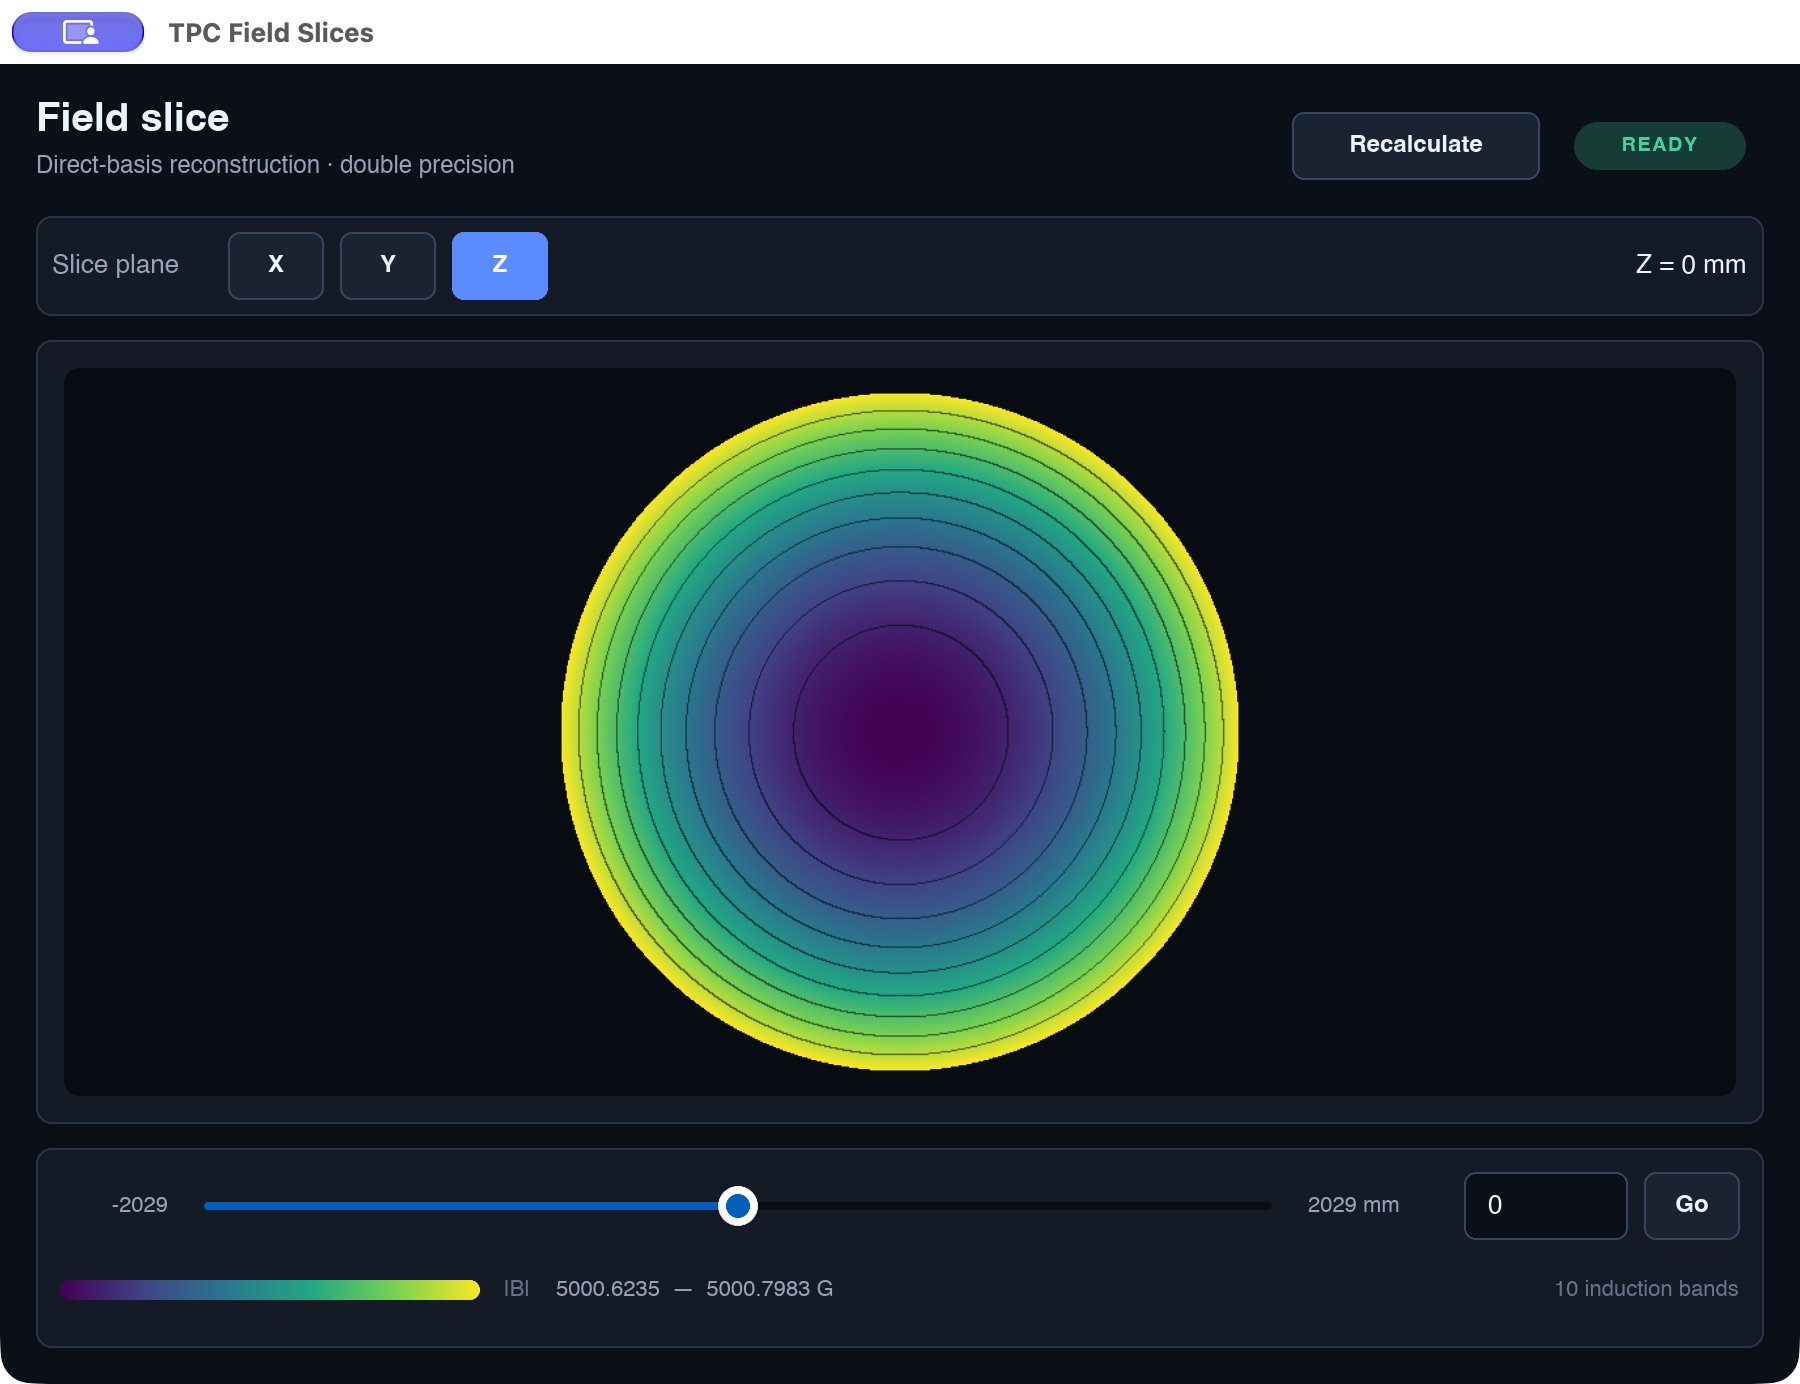
\includegraphics[width=\linewidth]{04-slice-z.jpg}
    \captionof{figure}{Поперечный срез $Z = 0$~мм.
      Диапазон $|\mathbf{B}|$ от 5000,6235 до 5000,7983~Гс.}
    \label{fig:slice-z}
  \end{minipage}
\end{center}

\begin{center}
  \begin{minipage}{115mm}
    \centering
    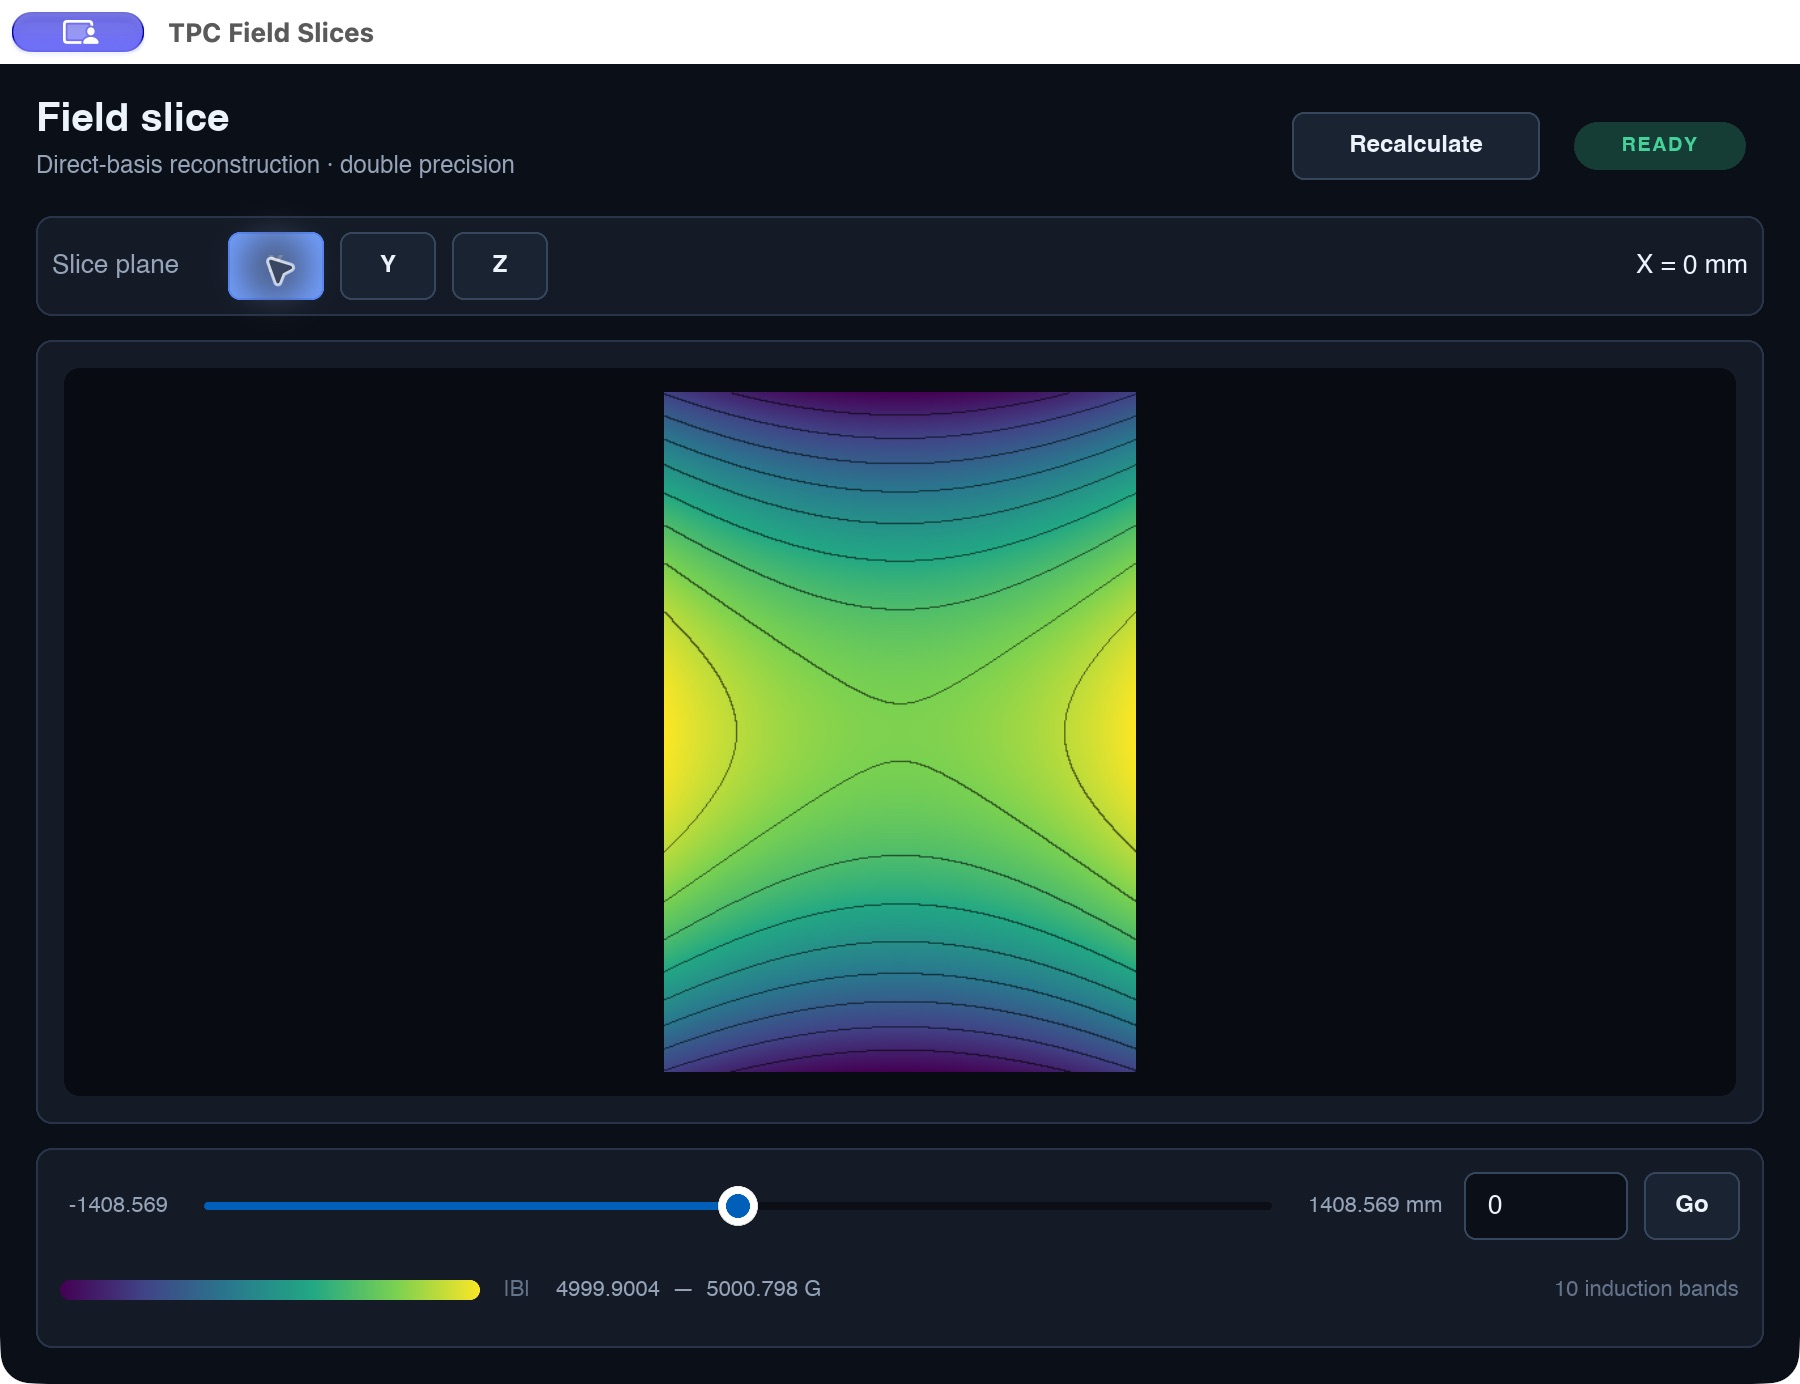
\includegraphics[width=\linewidth]{05-slice-x.jpg}
    \captionof{figure}{Продольный срез $X = 0$~мм.
      Диапазон $|\mathbf{B}|$ от 4999,9004 до 5000,798~Гс.}
    \label{fig:slice-x}
  \end{minipage}
\end{center}

\textbf{Результат работы.} Реализованы восстановление трёх компонент поля,
коррекция опорной карты, диагностика, срезы и экспорт.
Численная реализация проверена на тестовых полях.
Точность на реальной установке требует независимых контрольных измерений.

\textbf{Интерпретация срезов.} Разные диапазоны цветовой шкалы не позволяют
сравнивать неоднородность только по цвету. На поперечном срезе показанный
размах модуля составляет 0,1748~Гс, на продольном — 0,8976~Гс.
Это разности максимума и минимума на соответствующих срезах, а не ошибка
восстановления и не максимум отклонения во всём объёме.

\textbf{Дальнейшая проверка.} Для применения к установке необходимы
контрольные точки, не участвующие в подгонке коэффициентов, проверка
калибровки и ориентации датчиков, а также исследование сходимости
сеточной оценки экстремумов. Сопоставление с независимыми измерениями
позволит отделить ошибку выбранной модели от инструментальных погрешностей.

\end{document}
